\documentclass[fleqn]{scrartcl}
\usepackage[T1]{fontenc}
\usepackage[utf8x]{inputenc}
\usepackage{scrpage2}
\usepackage{paralist}
\usepackage{titling}
\usepackage{tabularx}
\usepackage{amsmath}
\usepackage{amsfonts}
\usepackage{amssymb}
\usepackage{mathtools}
\usepackage{ucs}
\usepackage[shortlabels]{enumitem}
\usepackage{graphicx}
\usepackage{listings}
\usepackage{tikz}
\usepackage{xcolor}

\definecolor{deepblue}{rgb}{0,0,0.5}
\definecolor{deepred}{rgb}{0.6,0,0}
\definecolor{deepgreen}{rgb}{0,0.5,0}

\lstset{
language=Python,
breaklines=true,
otherkeywords={self,nonlocal},             % Add keywords here
keywordstyle=\bfseries\color{orange},
emph={__init__},          % Custom highlighting
emphstyle=\color{deepred},    % Custom highlighting style
stringstyle=\color{deepgreen},
frame=tb,                         % Any extra options here
showstringspaces=false,            %
numbers = left
}

\pagestyle{scrheadings}
\clearscrheadfoot
\cfoot[\pagemark]{\pagemark}
\author{Tom Schmidt\\216204224 \and Stefan Poggenberg\\218100161 \and Samuel Schöpa\\216203821 \and Bjarne Hiller\\216203851}
\title{KI HA 1}
\date{18. Mai 2018}

\begin{document}
\maketitle
\section{Schiebepuzzles als Planungsproblem}
\subsection{3}
\begin{figure}[h!]
  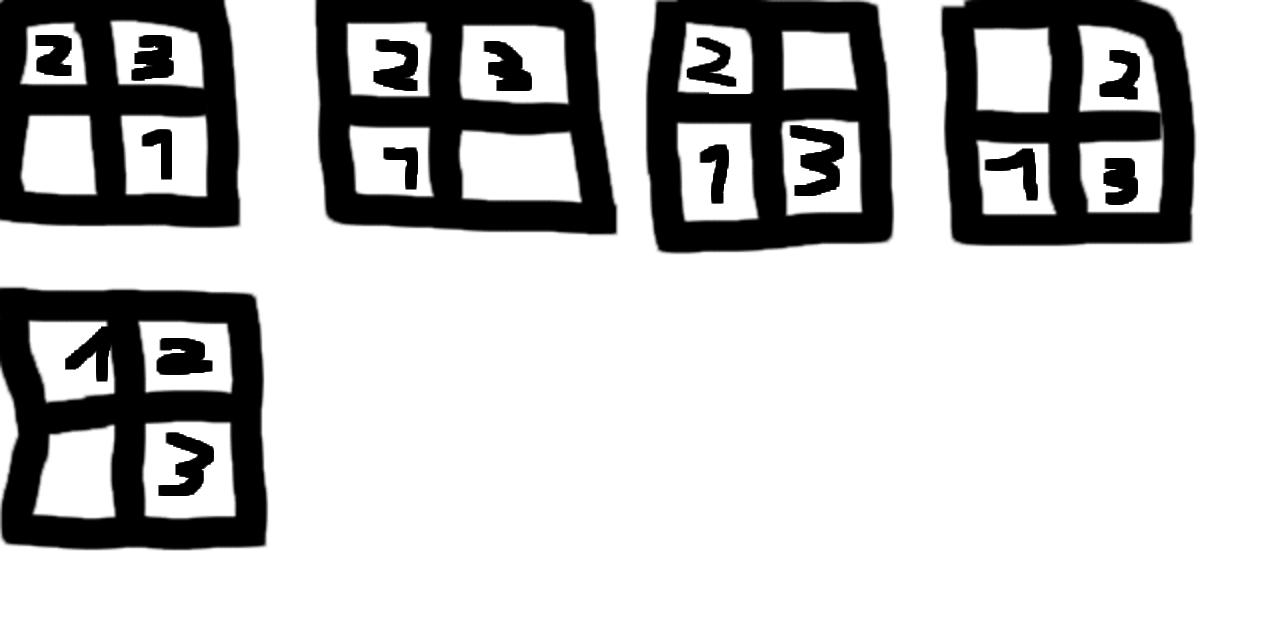
\includegraphics[width=\linewidth]{a2/3.PNG}
\end{figure}
\subsection{4}
  at(tile, position): Ist an gegebener Position gegebenes tile? \\
  empty(position): Ist auf der Position kein tile? \\
  neighbor(position, position): Liegen gegebene Positionen nebeneinander? \\
  move(tile, position): Bewege gegebenes tile auf gegebene Position. \\
\subsection{5}
\subsubsection{domain.pddl}
\lstinputlisting[firstline=1, lastline=25]{a2/domain.pddl}
\subsubsection{problem.pddl}
\lstinputlisting[firstline=1, lastline=32]{a2/problem.pddl}


\end{document}
